\documentclass[11pt]{amsart}

\usepackage{amsmath, amssymb, amsthm}
\usepackage{graphicx}
\usepackage{hyperref}
\usepackage{geometry}
\geometry{margin=1in}

\title{Phase Summation Patterns of Riemann Zeros}

\author{Rôtkiv Aynäsac}
\address{}
\email{}

\date{\today}

\begin{document}

\maketitle

\tableofcontents

\begin{abstract}
We investigate the partial sums 
\[
S(N)=\sum_{n\le N} e^{i\gamma_n},
\] 
where $\gamma_n$ denotes the imaginary parts of the nontrivial zeros of the Riemann zeta function. 
Although the statistical behavior of the spacings $\gamma_{n+1}-\gamma_n$ has been extensively studied and follows the Gaussian Unitary Ensemble (GUE) model, the global structure of the phases $e^{i\gamma_n}$ has received little systematic attention.

Our numerical experiments reveal several unexpected phenomena. 
First, the magnitude $|S(N)|$ remains confined to a narrow band for large $N$, with significantly suppressed growth compared to independent random phases. 
Second, $|S(N)|$ exhibits a quasi-periodic pattern, with prominent peaks occurring at intervals that cluster into discrete families. 
Third, the empirical distribution of peak spacings displays a distinctly multimodal structure. 

Together, these observations indicate nontrivial organization in the phase-sum
signal that merits further investigation. 
We discuss mechanisms including the deterministic phase drift from the Riemann--von Mangoldt law and potential interference effects arising from fine-structure fluctuations in the zeros. 
We present spectral analysis via FFT revealing distinct periodic components in the phase-sum interference pattern. 
The work is primarily exploratory and suggests directions for future theoretical investigation.
\end{abstract}


\section*{Introduction}

Let $\{\tfrac12+i\gamma_n\}_{n\ge1}$ denote the nontrivial zeros of the Riemann zeta function, ordered by increasing imaginary part.  
The statistical behavior of the sequence $(\gamma_n)$ has been the subject of extensive study for over fifty years.  
Montgomery's pair correlation conjecture \cite{Montgomery1973}, supported numerically by Odlyzko's computations \cite{Odlyzko1987,Odlyzko2001}, asserts that the local statistics of the normalized spacings
\[
\frac{\gamma_{n+1}-\gamma_n}{2\pi/\log(\gamma_n/2\pi)}
\]
match those of the Gaussian Unitary Ensemble (GUE) of random matrix theory.  
This connection has become a central pillar of analytic number theory, with deep implications for the distribution of primes and the explicit formula \cite{BerryKeating1999,Hejhal1994,ConreyGonek2001}.  

Despite this progress on local statistics, the behavior of the phases $e^{i\gamma_n}$ themselves has not been systematically investigated.  
While the differences $\gamma_{n+1}-\gamma_n$ exhibit GUE-type level repulsion, the absolute positions $\gamma_n \bmod 2\pi$ warrant examination.  
In particular, the complex partial sums 
\begin{equation}\label{eq:partialsum}
S(N)=\sum_{n\le N} e^{i\gamma_n},
\end{equation}
encode global interference patterns among zero phases and offer a novel lens on the global structure of the zeros.  
The quantity $S(N)$ may be viewed as a deterministic analogue of a two-dimensional random walk; understanding its behavior requires comparison with appropriate null models.

It has generally been assumed \cite{RudnickSarnak1996} that, after accounting for slowly changing density, the sequence $\{\gamma_n \bmod 2\pi\}$ is essentially equidistributed and uncorrelated at long range.  
Under this heuristic, one would expect $\mathbb{E}|S(N)|^2 \approx N$, corresponding to independent random phases.  
However, the gaps between successive $\gamma_n$ have a deterministic structure given by the Riemann--von Mangoldt law: the average gap is approximately $2\pi/\log(\gamma_n)$ for large $n$ \cite{Edwards1974}.  
This implies that the phase increments are not identically distributed, but follow a slowly changing (``chirped'') pattern.  
A refined null model should incorporate both this density trend and local GUE fluctuations.

In stark contrast to simple random-walk expectations, our numerical results indicate organized global behavior with significantly suppressed growth and emergent periodicities.  
The purpose of this work is to present a detailed numerical investigation of $S(N)$ and to characterize these unexpected phenomena.

As previewed above, we find that: 
\begin{itemize}
\item $|S(N)|$ remains confined to a narrow band with no long-term drift (contrary to $\sim \sqrt{N}$ growth of random-walk models).
\item The graph of $|S(N)|$ reveals quasi-periodic structure with prominent peaks at intervals clustering into discrete families.
\item The distribution of peak spacings is distinctly multimodal, indicating several preferred scales.
\end{itemize}

These patterns suggest the presence of long-range correlations among the phases not accounted for by GUE-based models focusing solely on local statistics.  
We discuss possible mechanisms and present both direct and spectral analyses of the data. 
This work is intended to document these phenomena and motivate future theoretical investigation.

This paper is organized as follows. Section~\ref{sec:results} presents our main numerical findings: behavior of $S(N)$ up to $N=10^4$ and analysis of peak spacings. 
We compare these findings to surrogate models to assess whether the observed structure is intrinsic to the actual zeros. 
Section~\ref{sec:fft} presents spectral (FFT) analysis of $|S(N)|$, interpreting prominent frequencies and their possible origins.  
We conclude with a summary and discussion of open questions.


\section{Results}
\label{sec:results}

In this section we present the numerical behavior of the partial sums $S(N)=\sum_{n\le N} e^{i\gamma_n}$, computed for the first $10^4$ Riemann zeros (with $\gamma_{10^4}\approx 28087$). 
All computations were performed in double precision using standard high-accuracy zero tables.  

\subsection{Global structure of $S(N)$}

Figure~\ref{fig:fases} displays the magnitude $|S(N)|$ for $1\le N\le 10^4$.
The most striking feature is the absence of diffusive growth: the values remain confined to a narrow vertical band (roughly $0$ to $5$) throughout the entire range.

\begin{figure}[h!]
\centering
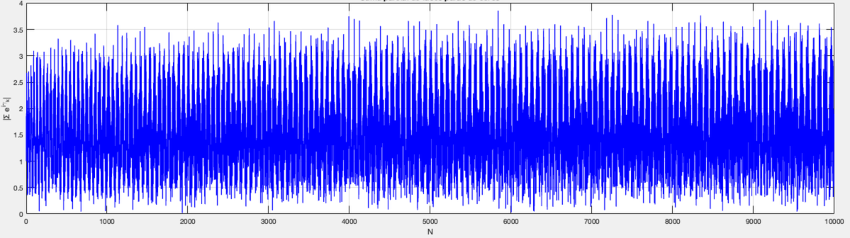
\includegraphics[width=0.85\textwidth]{fases.png}
\caption{Magnitude of the partial sums $S(N)=\sum_{n\le N} e^{i\gamma_n}$ for
$1\le N \le 10^4$. The values remain confined to a narrow vertical band around the horizontal axis, with dense oscillatory fluctuations and no visible long-term drift.}
\label{fig:fases}
\end{figure}

For an independent random walk with $N$ unit steps at uniformly random angles, the variance of the magnitude is $\mathbb{E}|S(N)|^2 = N$.  
However, the phase increments $\gamma_{n+1} - \gamma_n$ are not independent. 
Instead, they follow a deterministic trend: $\mathbb{E}[\gamma_{n+1}-\gamma_n] \approx 2\pi/\log(\gamma_n)$, which decreases slowly with $n$. 
This deterministic chirp represents a fundamental difference from the IID random-walk baseline.

The observed confinement of $|S(N)|$ within a narrow band indicates strong cumulative cancellations despite dense oscillatory fluctuations. 
This behavior differs markedly from simple models of independent phases.  
The mechanism underlying this confinement---whether arising from the density variation alone, from fine-structure fluctuations, or from long-range correlations---remains to be determined.

\subsection{Peak structure and quasi-periodicity}

A prominent feature of $|S(N)|$ is the appearance of pronounced peaks. 
To quantify this, we identify all local maxima of $|S(N)|$ exceeding $80\%$ of the global maximum and compute the distances between consecutive peaks.  
Let $1 \le N_1 < N_2 < \cdots < N_k \le 10^4$ denote the indices of these peaks, and define
\[
d_j = N_{j+1} - N_j.
\]

The histogram of $\{d_j\}$ is shown in Figure~\ref{fig:histo}. The distribution is distinctly multimodal: a dense cluster appears in the range $d_j \approx 5$--$15$, a second broader cluster around $d_j \approx 40$--$70$ (peaking near $50$), and a sparse tail beyond $100$.

\begin{figure}[h!]
\centering
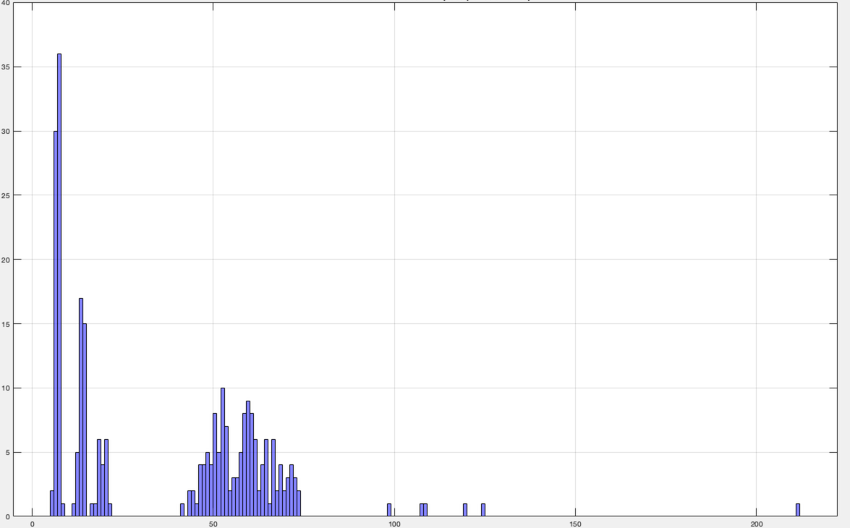
\includegraphics[width=0.85\textwidth]{Histo.png}
\caption{Histogram of distances $d_j$ between dominant peaks of $|S(N)|$ for
$N\le 10^4$. The distribution shows a pronounced cluster at short spacings (approximately $5$--$15$), a secondary cluster around $40$--$70$, and sparse larger gaps.}
\label{fig:histo}
\end{figure}

A heuristic based on the mean zero density suggests that peaks in $|S(N)|$ may occur when the accumulated phase is close to a multiple of $2\pi$. 
Since the average spacing of the $\gamma_n$ is $2\pi/\log \gamma_n$, the characteristic index spacing for a full $2\pi$ rotation is approximately
\begin{equation}\label{eq:logT}
\Delta N \approx \log \gamma_n \approx 10,
\end{equation}
in the range studied. This simple density-based argument explains the existence of a dominant short-spacing cluster.

The von Mangoldt model provides further insight. In the deterministic model $\tilde\gamma_n = 2\pi n/\log n$, the condition $\tilde\gamma_n \approx 2\pi k$ is satisfied at nearly regular intervals in $n$.  
The maxima of $|S(N)|$ occur at nearly constant separations, reflecting a well-defined fundamental period associated with the mean zero density.

For the actual Riemann zeros, this regular spacing persists but is modulated by additional fluctuations. 
These fluctuations broaden and split the short-spacing cluster and generate slower envelope modulations, giving rise to the secondary cluster around $d_j \approx 40$--$70$. 
The multimodal structure therefore indicates the coexistence of a density-driven fundamental periodicity with longer-range interference effects arising from the fine structure of the zeros.

\subsection{Comparison with surrogate models}

To assess whether the observed features could arise from simpler models, we compare $S(N)$ computed from the actual zeros with three surrogate sequences: 
(a) shuffled zeros, (b) a pure von Mangoldt model $\tilde\gamma_n = 2\pi n/\log n$, and (c) IID random phases $\phi_n \sim \mathrm{Uniform}[0,2\pi)$. 
Figure~\ref{fig:models} displays the results.

In the real-zero case, $|S(N)|$ remains bounded with structured quasi-periodic peaks. 
In contrast, the shuffled-zero and IID-phase models display diffusive growth, with $|S(N)|$ reaching values of order tens by $N=10^4$. 
The von Mangoldt model shows larger growth due to absence of local cancellations, but retains nearly constant peak spacings reflecting its deterministic structure.

None of the surrogate models reproduces the combination of bounded amplitude,
multimodal peak spacings, and spectral features observed for the actual
Riemann zeros.
This suggests that the observed phase-summation structure is associated with
the actual zero sequence rather than arising solely from the surrogate models
considered here.

\begin{figure}[h!]
\centering
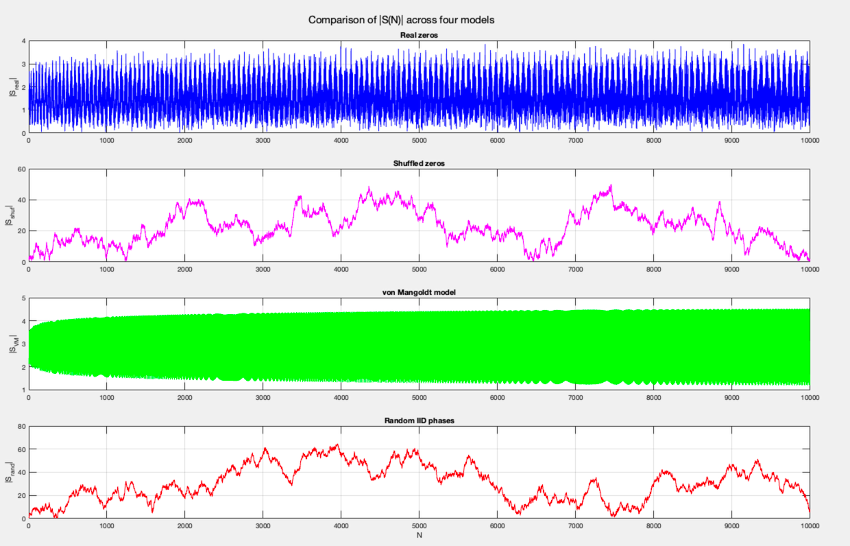
\includegraphics[width=0.85\textwidth]{4models.png}
\caption{Comparison of $|S(N)|$ for four phase sequences over $N\le 10^4$. 
\textbf{(Top)} Actual Riemann zeros (blue), exhibiting bounded amplitude with quasi-periodic peaks. 
\textbf{(Upper middle)} Shuffled real zeros (magenta), showing gradual diffusive growth. 
\textbf{(Lower middle)} Deterministic ``von Mangoldt'' model (green), derived from $\gamma_n \approx 2\pi n/\log n$, showing drift due to lack of local cancellations. 
\textbf{(Bottom)} i.i.d.\ uniform random phases (red), showing typical random-walk dispersion.}
\label{fig:models}
\end{figure}

Taken together, these comparisons indicate that the sequence $(e^{i\gamma_n})$ possesses a special structure not reproduced by any of the surrogate models.

\section{FFT Analysis of the Interference Pattern}
\label{sec:fft}

To further investigate the quasi-periodic behavior, we examined the frequency content of the sequence $|S(N)|$ by applying Fourier analysis. 
We treat $|S(N)|$ as a time series in the integer index $N$ and compute its discrete Fourier transform.  
This approach complements classical analyses of zero statistics by examining the cumulative phase interference pattern.

We computed the discrete Fourier transform of the zero-mean sequence $|S(N)| - \overline{|S(N)|}$ using the Cooley--Tukey FFT algorithm \cite{CooleyTukey1965}, 
with a Hann window applied to reduce spectral leakage.
From this we extracted the single-sided power spectral density $P(f)$ as a function of frequency $f$ (or equivalently, period $T = 1/f$).
We performed the same analysis on the $|S(N)|$ sequences of the three surrogate models for comparison. 
The amplitude spectra for the four cases are presented in Figure~\ref{fig:fftzeta}.

\begin{figure}[h!]
\centering
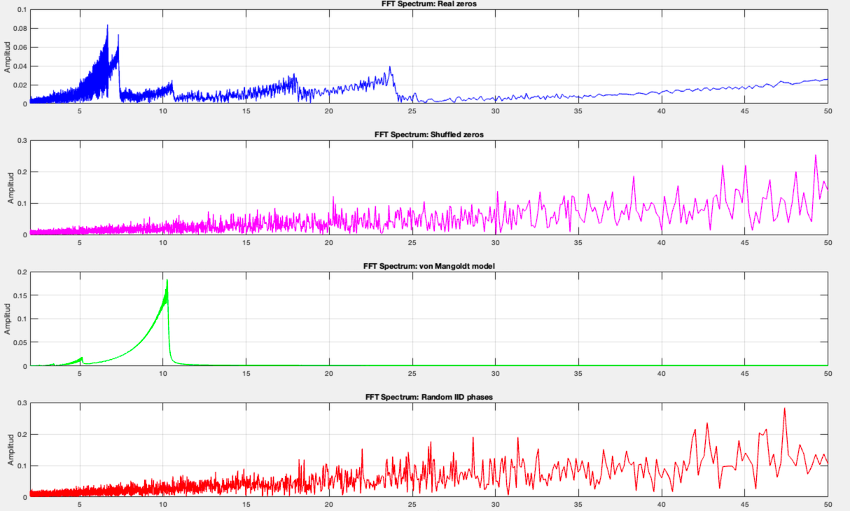
\includegraphics[width=0.85\textwidth]{FFTzeta.png}
\caption{FFT amplitude spectra of $|S(N)|$ (after removing the mean and applying Hann window) for the four models: 
actual Riemann zeros (blue, top), shuffled zeros (magenta, second), von Mangoldt model (green, third), and random i.i.d.\ phases (red, bottom). 
Horizontal axis shows equivalent period $T$ (in number of indices); only periods up to 50 are displayed. 
The real zeros display two sharp low-period peaks ($T\approx7$ and $T\approx10.5$) and a weaker resonance around $T\approx24$, whereas the surrogate sequences show no such distinct low-period peaks.}
\label{fig:fftzeta}
\end{figure}

For the von Mangoldt model (green curve, third panel), we observe a dominant frequency corresponding to period $T \approx 10.3$.  
This single sharp peak reflects the mean spacing of zeros: roughly 10 indices are needed for a full $2\pi$ phase rotation on average (consistent with $\log \gamma_n \approx 9$--$10$ in our range).  
This can be interpreted as the fundamental ``heartbeat'' of the Riemann zero phases in the absence of irregularity, in accord with the density-based spacing expectation \eqref{eq:logT}.  
The absence of other peaks in the von Mangoldt spectrum demonstrates that without fluctuations, only one scale of oscillation is present.

The actual Riemann zeros (blue spectrum, top panel) show more complex structure.  
Instead of one peak at $T\approx10$, the energy in the low-period region is split into at least two prominent peaks: a dominant one around $T\approx 7$ and a secondary one near $T\approx 10.5$.  
These correspond to the main clustering observed in the peak spacing histogram (Figure~\ref{fig:histo}). 
The presence of a strong component at $T\approx7$ (significantly shorter than the mean drift period) indicates an additional periodic modulation beyond the basic density chirp. 
This suggests that local fluctuations of the zeros induce a faster oscillatory pattern superimposed on the overall drift.  
In essence, the fundamental ``carrier'' frequency (period $\sim 10$) appears to have split into multiple modes due to the irregularities in $\gamma_n$. 

Additionally, the real-zero spectrum reveals a weaker but distinct resonance at period $T \approx 24$. 
This intermediate scale of modulation is absent from the von Mangoldt model. 
One possible explanation is that it reflects a beat frequency arising from
interference between the two dominant low-period components.
While intriguing, the precise origin of this resonance remains uncertain and warrants further investigation.

In contrast, the shuffled-zero and random-phase models (magenta and red spectra, second and bottom panels) show no significant low-period peaks.  
Their spectral energy is broadly distributed across higher frequencies, consistent with noise-like behavior.  
The distinctive periodic components observed for the real zeros are not generic to sequences with similar density or short-range statistics, confirming that they are tied to the specific fine structure of the zeta zeros.

To examine how spectral components evolve with $N$, we also performed a sliding-window FFT analysis on the real-zero sequence. 
The spectrogram in Figure~\ref{fig:FFTcont} (employing a window size of 1000 indices with 50\% overlap and Hann taper) shows the magnitude of the FFT as a function of period $T$ and the number of terms $N$ considered.  
Bright horizontal bands indicate persistent periodic components.  
A strong band corresponding to $T\approx10$ is present even for relatively small $N$ (around 1000) and persists through $N=9000$, gradually shifting downward (reflecting the slow decrease in $\Delta N$ as $\gamma_n$ increases). 
Simultaneously, a distinct band near $T\approx7$ emerges and persists, confirming that this faster oscillation is a robust feature across the range.  
Moreover, the spectrogram reveals higher-period structures (bands at $T\approx20, 30, 40$, etc.) particularly in the lower-$N$ region; these likely correspond to slower beats or higher-order interference patterns.

\begin{figure}[h!]
\centering
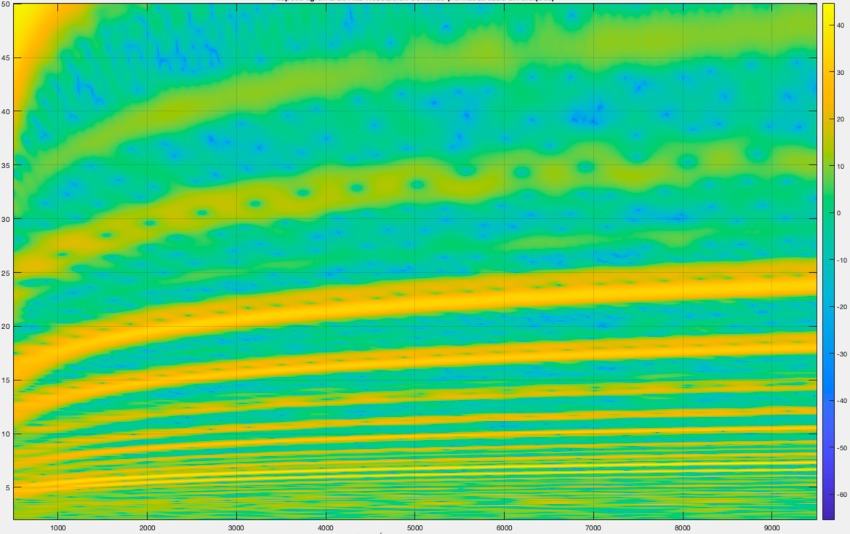
\includegraphics[width=0.85\textwidth]{FFTcontinuous.png}
\caption{Spectrogram (sliding FFT with 1000-point Hann window, 50\% overlap) of $|S(N)|$ for real Riemann zeros. 
Color intensity indicates spectral amplitude (dB) as functions of period $T$ (vertical axis, in index units, up to 50) and the number of terms $N$ (horizontal axis, from 1000 to 9000). 
Horizontal ridges correspond to persistent periodicities. 
A primary band (yellow) tracks from $T\approx15$ at $N=1000$ toward $T\approx10$ by $N=9000$, consistent with density-driven chirp. 
Another strong band appears around $T\approx7$, persisting across increasing $N$. 
Additional broader bands at higher periods (e.g., near 20--25 and 35--45 for smaller $N$) reflect slower interference effects.}
\label{fig:FFTcont}
\end{figure}

Several observations from the spectrogram merit discussion. 
First, the gradual downward drift of the fundamental band (from $\sim15$ to $\sim10$) mirrors the effect of Riemann--von Mangoldt density variation: as $\log \gamma_n$ slowly increases, the average periodicity shortens accordingly. 
Second, the stability of the $T\approx7$ band across the entire range suggests a structural periodicity beyond the mean spacing effect, potentially arising from systematic fine-structure fluctuations of the zeros.
Third, the faint but regular bands at higher periods (e.g., $T\approx20$--$30$ and $T\approx40$--$50$ for lower $N$) correspond to the secondary cluster of larger peak spacings (the 40--70 band in Figure~\ref{fig:histo}).  
These may represent slower modulation envelopes or beats arising from interplay between primary oscillations. 

In summary, the spectral analysis confirms that the $|S(N)|$ sequence contains distinct periodic components beyond the trivial mean spacing effect. 
These components, reflected in both the static spectrum and the spectrogram, underscore the existence of a structured interference pattern in the Riemann zero phases.

\section{Conclusions}

This numerical investigation reveals several unexpected features in the behavior of the partial sums 
\[
S(N)=\sum_{n\le N} e^{i\gamma_n}.
\]
While the local spacing statistics of the zeros follow the GUE model, the global patterns encoded in $S(N)$ exhibit structure that warrants attention.

We summarize our main findings:

\begin{enumerate}
\item \textbf{Suppressed growth of $|S(N)|$.}  
The magnitude remains confined to a narrow range, showing no diffusive growth with $N$, in stark contrast to expectations from independent random phases. 
The observed confinement implies strong cumulative cancellations among the exponential terms.

\item \textbf{Quasi-periodic peaks with multimodal spacing.}  
The partial sums exhibit pronounced peaks with distances clustering around specific values, notably $\sim 5$--$15$ (consistent with the density-driven scale $\log \gamma_n \approx 10$) and a secondary cluster around $40$--$70$. 
This multimodality indicates multiple interacting periodic components.

\item \textbf{Structure intrinsic to the zeros.}  
Control experiments with randomized or simplified sequences (shuffled zeros, pure density model, random phases) fail to reproduce the observed phenomena, indicating that the observed structure is tied to genuine properties of the zeta zeros.

\item \textbf{Spectral components in the interference pattern.}  
Fourier analysis reveals distinct periodic components beyond the trivial mean spacing effect. 
The dominant oscillation near $T\approx 10$ corresponds to density-driven phase drift; additional frequencies near $T\approx 7$ and a beat structure around $T\approx 24$ indicate multiple layers of periodicity not present in randomized models.

\end{enumerate}

The origin of the observed long-range structure remains open. Possible mechanisms include:
\begin{enumerate}
\item The slow variation of zero density (Riemann--von Mangoldt law), which creates a deterministic phase drift that may induce preferential cancellation patterns.
\item Fine-structure fluctuations in the zero sequence arising from arithmetic properties (such as coupling to prime distribution via the explicit formula), which could introduce additional correlations.
\item TAny structure detected in the phase-sum process is necessarily encoded in the
zero sequence itself and therefore does not represent independent spectral
data. However, such observables may reveal aspects of the organization of the
zeros that are not apparent in more commonly studied statistics.
\end{enumerate}

These observations raise several questions for future investigation:
\begin{itemize}
\item Do the phases $\gamma_n \bmod 2\pi$ satisfy nontrivial equidistribution laws with hidden correlations or constraints?
\item Can the observed quasi-periodicity be derived from the explicit formula or other analytic properties of $\zeta(s)$?
\item Is there a dynamical or geometric model (in the spirit of the Hilbert--Pólya conjecture or quantum chaos analogies) that reproduces the behavior of $S(N)$?
\item How do the phenomena evolve at larger $N$? Do they persist, strengthen, or fade?
\end{itemize}

Addressing these questions will require extending current frameworks and developing new analytic and computational techniques. 
In particular, extending the numerical investigation to higher $N$ (using existing zero databases) and constructing refined null models incorporating both the von Mangoldt density and GUE-like local fluctuations would illuminate whether the observed structure represents a genuine long-range phenomenon intrinsic to the Riemann zeros.

The phase-sum function $S(N)$ offers a novel perspective on the global structure of the Riemann zeros. 
The patterns documented here suggest that significant structure may yet be hidden in the cumulative interference of zero phases, warranting both further numerical exploration and theoretical investigation.

\begin{thebibliography}{99}

\bibitem{Montgomery1973}
H.~L.~Montgomery, 
\emph{The pair correlation of zeros of the zeta function}, 
Proc. Symp. Pure Math. \textbf{24} (1973), 181--193.

\bibitem{Odlyzko1987}
A.~M.~Odlyzko, 
\emph{On the distribution of spacings between zeros of the zeta function}, 
Math. Comp. \textbf{48} (1987), 273--308.

\bibitem{Odlyzko2001}
A.~M.~Odlyzko, 
\emph{The $10^{20}$-th zero of the Riemann zeta function and 70 million of its neighbors}, 
preprint (2001).

\bibitem{Mehta2004}
M.~L.~Mehta, 
\emph{Random Matrices}, 
3rd ed., Elsevier/Academic Press, 2004.

\bibitem{BerryKeating1999}
M.~V.~Berry and J.~P.~Keating, 
\emph{The Riemann zeros and eigenvalue asymptotics}, 
SIAM Rev. \textbf{41} (1999), 236--266.

\bibitem{Hejhal1994}
D.~A.~Hejhal, 
\emph{On the triple correlation of zeros of the zeta function}, 
Int. Math. Res. Not. (1994), 293--302.

\bibitem{ConreyGonek2001}
J.~B.~Conrey and S.~M.~Gonek, 
\emph{High moments of the Riemann zeta-function}, 
Duke Math. J. \textbf{107} (2001), 577--604.

\bibitem{RudnickSarnak1996}
Z.~Rudnick and P.~Sarnak, 
\emph{Zeros of principal $L$-functions and random matrix theory}, 
Duke Math. J. \textbf{81} (1996), 269--322.

\bibitem{Edwards1974}
H.~M.~Edwards, 
\emph{Riemann's Zeta Function}, 
Academic Press, 1974.

\bibitem{CooleyTukey1965}
J.~W.~Cooley and J.~W.~Tukey, 
\emph{An algorithm for the machine calculation of complex Fourier series}, 
Math. Comp. \textbf{19} (1965), 297--301.

\end{thebibliography}

\appendix

\section{Code for Data Generation and Analysis}
\label{app:code}

{\small 
\begin{verbatim}
%% Partial sums computation and comparison
N     = length(gamma);
n_vec = (1:N).';

% Real zeros
Z_real   = exp(1i * gamma);
S_real   = cumsum(Z_real);
abs_real = abs(S_real);

% Shuffled zeros
gamma_shuf = gamma(randperm(N));
Z_shuf     = exp(1i * gamma_shuf);
S_shuf     = cumsum(Z_shuf);
abs_shuf   = abs(S_shuf);

% Von Mangoldt model
gamma_vm        = zeros(N,1);
idx_valid       = n_vec >= 3;
gamma_vm(idx_valid) = 2*pi * n_vec(idx_valid) ./ log(n_vec(idx_valid));
Z_vm    = exp(1i * gamma_vm);
S_vm    = cumsum(Z_vm);
abs_vm  = abs(S_vm);

% Random IID phases
phi_rand = 2*pi*rand(N,1);
Z_rand   = exp(1i * phi_rand);
S_rand   = cumsum(Z_rand);
abs_rand = abs(S_rand);

%% FFT analysis with Hann window
real_center = abs_real - mean(abs_real);
shuf_center = abs_shuf - mean(abs_shuf);
rand_center = abs_rand - mean(abs_rand);
abs_vm_valid = abs_vm(idx_valid);
vm_center    = abs_vm_valid - mean(abs_vm_valid);

% Apply Hann window
N_real = length(real_center);
N_vm   = length(vm_center);
win_real = hann(N_real)';
win_vm   = hann(N_vm)';

real_windowed = real_center .* win_real;
shuf_windowed = shuf_center .* hann(length(shuf_center))';
rand_windowed = rand_center .* hann(length(rand_center))';
vm_windowed   = vm_center .* win_vm;

% FFT computation
Y_real = fft(real_windowed);
Y_shuf = fft(shuf_windowed);
Y_vm   = fft(vm_windowed);
Y_rand = fft(rand_windowed);

% Power spectral density
P_real = abs(Y_real(1:ceil(N_real/2))).^2 / (N_real * sum(win_real.^2));
P_shuf = abs(Y_shuf(1:ceil(N_real/2))).^2 / (N_real * sum(hann(length(shuf_center)).^2));
P_rand = abs(Y_rand(1:ceil(N_real/2))).^2 / (N_real * sum(hann(length(rand_center)).^2));
P_vm   = abs(Y_vm(1:ceil(N_vm/2))).^2 / (N_vm * sum(win_vm.^2));
\end{verbatim}
}

\end{document}
